\documentclass[12pt]{article}


\usepackage{amsmath}
% \usepackage{german}
\usepackage[pdftex]{graphicx}
\usepackage{wrapfig}
\DeclareMathOperator\sgn{sgn}

%\graphicspath{{/home/ritz/Teaching/fcn/fig/}}

%----------------- layout ----------------------------------------

\oddsidemargin=0in
\textwidth=6in
\topmargin=-0.7in
\textheight=9.5in
\baselineskip=16pt
\font\mittel=cmr17
\font\roman=cmr12
\font\klein=cmr9
\font\mgross=cmr10
\newfont{\CAP}{cmcsc10 scaled 900}
\pagestyle{empty}
\parindent=0mm

%----------------- macros ----------------------------------------
\newcommand{\conc}[1]{[{\rm C}]_{\text{#1}}}
\newcommand{\units}[1]{\text{#1}}
\newcommand{\kalium}{$\text{K}^+$}
\newcommand{\natrium}{$\text{Na}^+$}
\newcommand{\chlor}{$\text{Cl}^-$}
\newcommand{\wasser}{$\text{H}_2\text{O}$}
\newcommand{\tderiv}[1]{\frac{\mathrm{d}#1}{\mathrm{d}t}}
%-----------------------------------------------------------------


\begin{document}

\parbox{2cm}{

\includegraphics[width=1.8cm]{bccnlogo.pdf}
}
\parbox{11cm}{
\begin{center}
\large HUMBOLDT-UNIVERSIT\"AT \hskip 0.1 cm ZU \hskip 0.1 cm BERLIN
\vskip 0.1 true cm
\mgross BERNSTEIN CENTER FOR COMPUTATIONAL NEUROSCIENCE
\end{center}
}
\parbox{2cm}
{
\hfill

\includegraphics[width=1.8cm]{hublogo.pdf}
}

\vskip 0.6 true cm

\leftline{\CAP Humboldt-Universit\"at zu Berlin 
\hfill Phone: 030/2093-9110}
\leftline{\CAP Philippstr. 13 House 6
              \hfill Fax: 030/2093-6771}
\leftline{\CAP \hfill webpage: http://www.bccn-berlin.de/}


\vskip 0.8 true cm
\centerline{\bf Models of Neural Systems, WS 2010/11}
\centerline{\bf Computer Practical 6}
\centerline{Solutions to hand in on: December, 6th, 2010}

\vskip 0.8 true cm
%----------- EXERCISES BEGIN ---------------------%

{\bf Exercises}

\vskip 0.8 true cm
% \begin{enumerate}

%\item 
\textbf{1. Synaptic current} 

Simulate a linear membrane that receives an external synaptic input:
%Equation can be also modified by including synaptic conductances in the membrane current:

\begin{equation}
\tau_m \tderiv{V(t)}=-V(t)+E_m-r_m\,I_{syn}(t)+R_m I_e,
\label{eq:membrane}
\end{equation} 
where $I_{syn}(t)=g_{syn}(t)(V(t)-E_{syn})$ is the post-synaptic
current, $g_{syn}(t)$  is the synaptic conductance. The change of
the conductance due to a pre-synaptic spike can be described by:

\begin{equation}
 g_{syn}(t)= 
\begin{cases} g_{max}\,t/\tau_{syn}\exp\left(-t/\tau_{syn}\right) & \text{if $t\geq0$,}
\\
0 &\text{if $t<0$.}
\label{eq:synaptic_conductance}
\end{cases}
\end{equation} 
 
 Here take $\tau_{syn}$=10 ms, $\tau_m$=10 ms, $r_m=1\,\mathrm{\Omega m^2}$,
$g_{max}=0.5\,\mathrm{S/m^2}$, $E_m=-80$ mV, $R_m I_e=0$mV.
 
\begin{enumerate}
    \item \label{ex:syncurrent} Plot the following curves for a single
        pre-synaptic spike in one figure:
        synaptic conductance $g_{syn}(t)$, synaptic current
        $I_{syn}(t)$, membrane current $I_m(t)=(V(t)-E_m)/r_m$,
        membrane potential $V(t)$.
        Consider inhibitory ($E_{syn}=-100\,\mathrm{mV}$) and excitatory
        ($E_{syn}=0\,\mathrm{mV}$) synapses separately.
        \item \textit{Shunting inhibition}. In vivo neurons are constantly
        bombarded by balanced excitatory and inhibitory inputs. In order to
        model the background activity, assume that in addition to the
        time-dependent synaptic conductance (Equation
        \ref{eq:synaptic_conductance}) the membrane receives tonic inhibitory
        and excitatory inputs which can be best described by constant
        conductances. The total synaptic current equals:
        $$I_{syn}=g_{syn}(t)(V(t)-E_{syn})+g_{exc}(V(t)-E_{exc}) +
        g_{inh}(V(t)-E_{inh})$$
        with $g_{exc}= 0.5 \mathrm{S/m^2}$ and $g_{inh}= 2.0 \mathrm{S/m^2}$ .
        Show that the resting potential of the membrane doesn't change due to
        the tonic synaptic inputs. Simulate the membrane response to a
        transient excitatory synaptic input and compare it with the result from
        Exercise 1a. How would you explain the differences?

 \end{enumerate}
 
  \newpage
% \item 
  \textbf{2. Synaptically coupled IF neurons.}

        \begin{wrapfigure}{r}{0.25\textwidth}
          \centering
          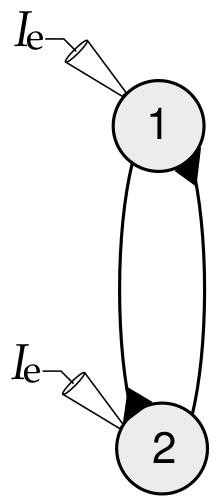
\includegraphics[width=0.18\textwidth]{coupledIFs.png}
          \caption{Mutually coupled Integrate-and-fire neurons.}
          \noindent \hrulefill
          \label{fig:CoupledIFs}
        \end{wrapfigure}

    The smallest possible recurrent network consists of two interconnected
    neurons, as depicted in Figure~\ref{fig:CoupledIFs}. For simplicity, we
    assume both synapses to be of the same type (excitatory or inhibitory) and
    of equal strength ($g_{max}$).
    
    \begin{enumerate}
     \item Implement this model with Integrate-and-fire neurons: the membrane
    voltage development of each neuron is described
    by equation~\ref{eq:membrane}, with the additional property of being reset
    to $V_{reset}=-80$mV, when it exceeds the threshold potential
    $V_\mathrm{th}=-54\,\mathrm{mV}$ (see exercise 3 of sheet 5). The time $t$
    of the synaptic conductance in equation~\ref{eq:synaptic_conductance} of
    each neuron is measured relative to the last spike (membrane reset) of
    the other (presynaptic) neuron. Use for both model neurons $E_m$ = $-70$mV,
    $r_m= 1\,\mathrm{\Omega m^2}$, $g_{max} = 0.05\,\mathrm{S/m^2}$, $R_m I_e
    = 25$mV, $\tau_{syn} = 10$ms, $\tau_m=10$ms.
    \item Plot and compare the membrane potential development for the two
          neurons in case of excitatory and inhibitory synaptic interactions.
          Comment and explain the observed behavior.
    \item Analyze how the pattern of firing for the two neurons
          depends on the strength ($g_{max}$) and time
          constant ($\tau_{syn}$) of the reciprocal synaptic connection for both
          inhibitory and excitatory interactions. Plot and comment
          on characteristic cases.
% (see Van Vreeswijk et al, 1994).
    \end{enumerate}

 {\bf 3. Report.} Submit the plain source code files for all exercises
         and a report containing the source code, all plots and answers to the
         questions asked.

% \item \textbf{Potassium channel}
% 
%     The gate model was first introduced by Hodgkin and Huxley to describe voltage and
% time dependence of ion conductances in the squid axon. Today it is still the
% standard model of the ion current flow through transmembrane channels. One of
% its main assumptions is that the probability of opening and closing of an ion
% gate is described by the first-order kinetic equation: 
% \begin{equation}
%     \tderiv{n}=\alpha_n(V)(1-n)-\beta_n(V)n
%     \label{eq:activation}
% \end{equation}
% 
% where $\alpha_n(V)$ and $\beta_n(V)$ are voltage-dependent transition rates.
% 
%     The potassium current in the Hodgkin-Huxley model is given by:
%     \begin{equation}
%         I_K=\bar{g}_{K} n^4 (V-E_K)
%         \label{eq:potassium}
%     \end{equation}
% 
%     where $E_K=-77\,\mathrm{mV}$ is the reversal potential and $\bar{g}_K=36\,\mathrm{mS/cm^2}$ is the maximum conductance. Rates $\alpha_n(V)$ and $\beta_n(V)$ are given by:
%     \begin{equation}
%         \alpha_n(V)=\frac{0.01(V+55)}{1-\exp(-0.1(V+55))},\quad \beta_n(V)=0.125\exp(-0.0125(V+65)),
%     \end{equation}
% where $V$ is expressed in mV, and $\alpha_n$ and $\beta_n$ are both expressed in units of ms$^{-1}$.
%     \begin{enumerate}
%         \item Write Python functions defining $\alpha_n(V)$ and $\beta_n(V)$.
%         \item \label{ex:stedy-state} Plot the steady-state activation $n_\infty(V)=\alpha_n(V)/(\alpha_n(V)+\beta_n(V))$ and the activation time constant $\tau_n(V)=1/(\alpha_n(V)+\beta_n(V))$ in a voltage range of $-150\,\mathrm{mV}\leq V \leq 150\,\mathrm{mV}$.
%         \item \textit{Voltage clamp}. Calculate the current responses
%             $I_K$ to voltage steps under voltage-clamp conditions:
%             \begin{equation*}
% V(t)= 
% \begin{cases} V_c & \text{if $t\geq2$ ms,}
% \\
% -65\,\mathrm{mV} &\text{otherwise.}
% \end{cases}
% \end{equation*}
% with the initial condition $n(t=0)=0.3177$. Plot $I_K$ as a function of time. Repeat the simulation for different values of clamping voltage $V_c$ from the range  $[-100\,\mathrm{mV}, -40\,\mathrm{mV}]$. What can be learnt from this experiment? What is the predicted effect of the potassium current on the membrane potential?   Explain the obtained results referring to the plots of the activation variables $n_\infty$ and $\tau_n$.
%         \item \textit{Current-voltage relation}. Plot the I-V relation for the instantaneous and steady-state potassium current.
%     \end{enumerate}
% \end{enumerate}

%----------- EXERCISES END -----------------------%

\vfill
\centerline{\CAP Contact}
\CAP

\begin{tabular}{lll}
Urs Bergmann & Phone: 2093-8924 & Email:
urs.bergmann(at)biologie.hu-berlin.de \\
Matthias Guggenmos & & Email: matthias.guggenmos(at)bccn-berlin.de \\
Richard Kempter \hfill & Phone: 2093-8925 \hfill & Email:
r.kempter(at)biologie.hu-berlin.de \\
%Robert Schmidt & Phone: 2093-8926 & Email: r.schmidt(at)biologie.hu-berlin.de
%\\
%Bartosz Telenczuk & Phone: 2093-8838 & Email:
%b.telenczuk(at)biologie.hu-berlin.de \\
\end{tabular}

\end{document}
 
